\section{Band topology: Wilson loops, Chern numbers, and time reversal}
\label{sec:topology}

The overlap matrices used for Wannier construction also contain the geometry
of an isolated band subspace. Following established hybrid-Wannier and
Wilson-loop formulations~\cite{Soluyanov2011,Gresch2017}, the native analysis
in \CPtwoK{} evaluates Berry phases, hybrid Wannier charge centers, the
$\mathbb Z_2$ invariant of a time-reversal-invariant plane, and the first
Chern number $C_1$. The native analysis evaluates Wilson loops and
topological invariants directly from Gaussian-basis Bloch-state overlaps,
without requiring Z2Pack or a maximally localized Wannier representation.
Z2Pack remains an optional external analysis route and a complementary
validation tool. Its adapter supplies the same first-principles overlaps
to an external implementation with its own line and surface sampling.
Neither route requires a fitted tight-binding Hamiltonian.

\subsection{Interband geometry and Berry curvature}
The velocity and dipole matrix elements in
Eqs.~\eqref{eq:bloch-velocity} and \eqref{eq:interband-dipole} also connect
the local-orbital representation to band geometry. For a nondegenerate
band, the moment implementation evaluates the interband expression
\begin{equation}
 \begin{split}
 \Omega^\gamma_n(\bk)
 &=2\,\operatorname{Im}\sum_{m\ne n}
 d^\alpha_{nm}(\bk)d^\beta_{mn}(\bk)\\
 &=2\,\operatorname{Im}\sum_{m\ne n}
 \frac{v^\alpha_{nm}(\bk)v^\beta_{mn}(\bk)}
 {(\varepsilon_{n\bk}-\varepsilon_{m\bk})^2},
 \end{split}
 \label{eq:berry-curvature-dipoles}
\end{equation}
where $(\alpha,\beta,\gamma)$ is a cyclic permutation of $(x,y,z)$.
This equation uses the sign convention of the moment output.
Comparisons with overlap-based phases require matching the phase and
surface-orientation conventions. With Cartesian reciprocal coordinates,
$\Omega^\gamma_n$ has units of length squared. The formula reveals why
small avoided crossings can produce sharply localized curvature and why
band-energy convergence alone does not establish convergence of this
observable. The band sum, AO basis, and reciprocal-space sampling require
separate convergence checks.

The product in Eq.~\eqref{eq:berry-curvature-dipoles} is invariant under
independent phase changes of nondegenerate eigenstates. At an exact
degeneracy, however, the individual-band assignment is not invariant
under rotations within the degenerate subspace, and division by the
vanishing energy difference is not defined. An isolated group of bands
must instead be treated through its projector or matrix-valued
connection. The Wilson construction below implements this subspace
viewpoint without resolving arbitrary eigenvectors within the group.
The interband expression describes the implemented finite-basis moment
representation and is not by itself a proof of complete-basis curvature
or an integer Chern number. Nor does this geometric quantity constitute
an implementation of anomalous Hall transport, which is distinct from
the dissipative response in Section~\ref{sec:kubo}.

\subsection{Directed overlaps and Wilson loops}
Consider a closed directed path $\bk_0,\ldots,\bk_{L}$ with
$\bk_L=\bk_0+\bG$ and links $\bb_j=\bk_{j+1}-\bk_j$.
For $N_{\mathrm{occ}}$ occupied states, each link is the square matrix in
Eq.~\eqref{eq:wannier90-mmn-definition}. In the Gaussian representation,
its AO operator is explicitly
\begin{equation}
 O_{\mu\nu}(\bk+\bb;\bb)=
 \sum_{\bR}e^{\ii(\bk+\bb)\cdot\bR}
 \langle\phi_{\mu\bm 0}|e^{-\ii\bb\cdot\br}|\phi_{\nu\bR}\rangle .
 \label{eq:topology-ao-operator}
\end{equation}
Here $\phi_{\mu\bR}(\br)=\phi_\mu(\br-\bR)$ denotes an
individual localized orbital, not a Bloch sum. The zero-step limit
recovers $S(\bk)$. At finite displacement, however,
this is a directed cross-k operator, not a Hermitian matrix at one k-point.
Its construction retains ordered atom pairs, image-cell phases, and the
same periodic atomic images as the Hamiltonian. Consequently, neither
$C^\dagger(\bk)C(\bk+\bb)$ nor replacement of the operator by $S(\bk)$
represents the required overlap. Reciprocal-boundary links retain their
integer $\bG$ shift, implementing
$u_{n,\bk+\bG}(\br)=e^{-\ii\bG\cdot\br}u_{n\bk}(\br)$ in a consistent
boundary gauge.

At finite sampling the occupied-subspace overlap need not be unitary. Each
link is factorized and replaced by its unitary polar factor,
\begin{equation}
 M_j=U_j\Sigma_j V_j^\dagger,\qquad
 Q_j=U_jV_j^\dagger,\qquad
 \mathcal W=Q_0Q_1\cdots Q_{L-1}.
 \label{eq:topology-wilson}
\end{equation}
The smallest singular value of $M_j$ diagnoses loss of continuity or an
inadequately resolved subspace. A rank-deficient link is rejected. For a
unitary change of occupied-band basis $C_j\mapsto C_jG_j$, the link and
closed product transform as
\begin{equation}
 Q_j\mapsto G_j^\dagger Q_jG_{j+1},\qquad
 \mathcal W\mapsto G_0^\dagger\mathcal W G_0 .
 \label{eq:topology-gauge}
\end{equation}
Thus the Wilson spectrum is gauge invariant although individual overlaps
are not. With the path and phase convention used here,
\begin{equation}
 \lambda_n(\mathcal W)=e^{2\pi\ii\bar x_n},\qquad
 \bar x_n=\frac{\arg\lambda_n}{2\pi}\pmod 1,\qquad
 \gamma=\arg\det\mathcal W .
 \label{eq:topology-centers}
\end{equation}
The $\bar x_n$ are the hybrid Wannier charge centers in reduced units,
and $\gamma$ is the total loop phase in this convention. Reversing the loop
reverses the eigenphases. The absolute center origin follows the atomic and
cell-origin convention, whereas the topological classification does not.

For spinful time-reversal symmetry, loops spanning half a reciprocal plane
connect two time-reversal-invariant boundaries. The parity of partner
exchange in the center spectrum determines the two-dimensional invariant.
The largest-gap construction tracks the center $z_\ell$ of the largest
gap between adjacent centers on each sampled loop and counts crossings
between successive loops~\cite{Soluyanov2011,Gresch2017}, giving
\begin{equation}
 \nu=N_{\mathrm{cross}}\pmod 2 .
 \label{eq:topology-z2}
\end{equation}
Loop resolution and transverse sampling are refined together. Acceptance
uses center displacements, neighboring-loop gap separation, boundary
Kramers pairing, and stable parity. The occupied rank is fixed and separated
from conduction states throughout the sampled surface.

On a closed full reciprocal-space surface, $C_1$ is obtained instead from
the winding of the determinant Wilson phase. With
$\gamma_\ell=\arg\det\mathcal W_\ell$ and a periodic transverse index,
the discrete estimate in the present orientation convention is
\begin{equation}
 C_1^{\mathrm{mesh}}=\frac{1}{2\pi}\sum_\ell
 \operatorname{Arg}\exp\!\left[\ii(\gamma_{\ell+1}-\gamma_\ell)\right].
 \label{eq:topology-c1}
\end{equation}
The phase increments must be resolved under refinement, and the final
transverse boundary must be sewn to the initial one. Unlike the
time-reversal half-plane construction, this calculation covers a full
closed surface and does not require time-reversal symmetry. The native
implementation checks closure and stable winding under refinement and
retains the unrounded winding alongside the integer candidate.

In \CPtwoK{}, explicit fractional k-points and directed connections are
read from a \texttt{.nnkp} file with \texttt{KPOINTS\_SOURCE NNKP}, or
generated internally with \texttt{KPOINTS\_SOURCE WILSON}.
\texttt{WILSON\_LOOP} evaluates a loop, \texttt{Z2} selects the
half-plane analysis, and \texttt{CHERN} selects the full-surface $C_1$
analysis. The converged SCF potential is held fixed while the
post-SCF points are diagonalized. The integration mesh defining the density
and the ordered paths probing its band topology are distinct objects.
Spin--orbit coupling (SOC) enters through a second-variational spinor
Hamiltonian built from the scalar states and pseudopotential SOC matrix
elements. For spinor coefficients the link is
\begin{equation}
 M_j=C_{j,\uparrow}^\dagger O_jC_{j+1,\uparrow}
       +C_{j,\downarrow}^\dagger O_jC_{j+1,\downarrow},
 \label{eq:topology-spinors}
\end{equation}
and band selection refers to this spinor spectrum.

This application makes the role of symmetry particularly clear. Scalar
irreducible-mesh weights cannot replace an ordered Wilson product. A path
requires explicit states at its points or their symmetry reconstruction
with all orbital rotations, spin transformations, and boundary phases.
The native explicit-path calculation obtains these states by diagonalizing
the fixed-potential problem at the requested points. It therefore
complements symmetry-reduced SCF quadrature while retaining the complete
neighbor connectivity needed for a gauge-covariant observable.

Figure~\ref{fig:topology} demonstrates the calculation using small test
systems: a periodic neon reference and buckled stanene, a representative quantum spin Hall
system~\cite{Xu2013}. The computed invariants are $\nu=0$ and $\nu=1$,
respectively. The sampling-converged stanene surface contains 193 loops with 192
points per loop. Native and Z2Pack analysis of the same polar-unitarized
overlaps agree in the Wilson eigenvalues to $8\times10^{-14}$. A separately
adaptive Z2Pack-driven calculation also yields $\nu=1$. Operator-level
checks independently test the zero-step metric, reverse-link adjoint
identity, and displaced atomic centers. These complementary tests connect
the local Gaussian integral representation to the global topology of the
occupied bands. Inputs, sampling parameters, and figure data are given in
the Supporting Information and accompanying calculation records.

\begin{figure}[tbp]
 \centering
 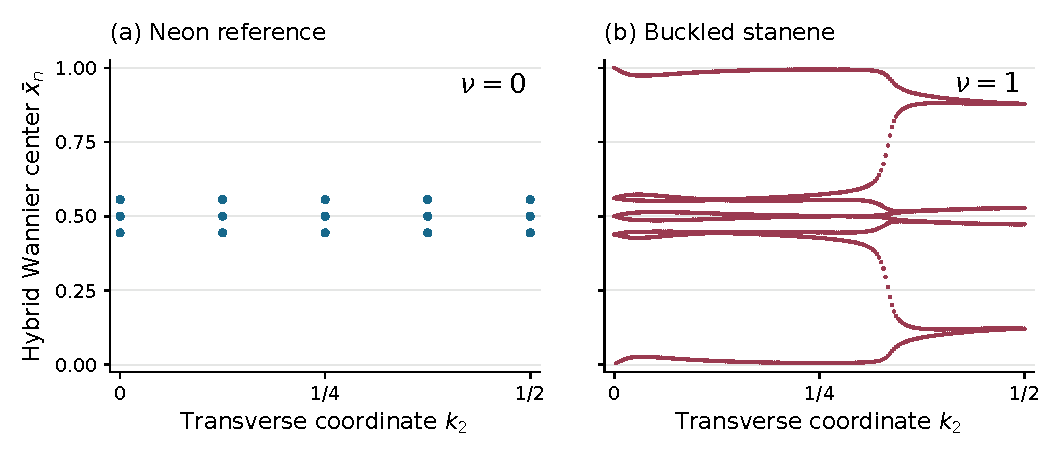
\includegraphics[width=\linewidth]{figures/wilson-centers.pdf}
 \caption{Wilson-loop test and demonstration calculations for
 (a) a periodic neon reference and
 (b) buckled stanene. Points are the computed hybrid Wannier centers in
 reduced units. Degenerate centers coincide. Each loop winds once along
 the first reciprocal coordinate, while the transverse coordinate spans
 $0\leq k_2\leq 1/2$ at $k_3=0$. The neon and stanene surfaces contain
 five and 193 loops, respectively, and yield $\nu=0$ and $\nu=1$.
 All eight occupied spinor centers are shown.}
 \label{fig:topology}
\end{figure}
